\documentclass[border=10pt]{standalone}
\usepackage{pgfplots}
\pgfplotsset{compat=1.18}
\begin{document}
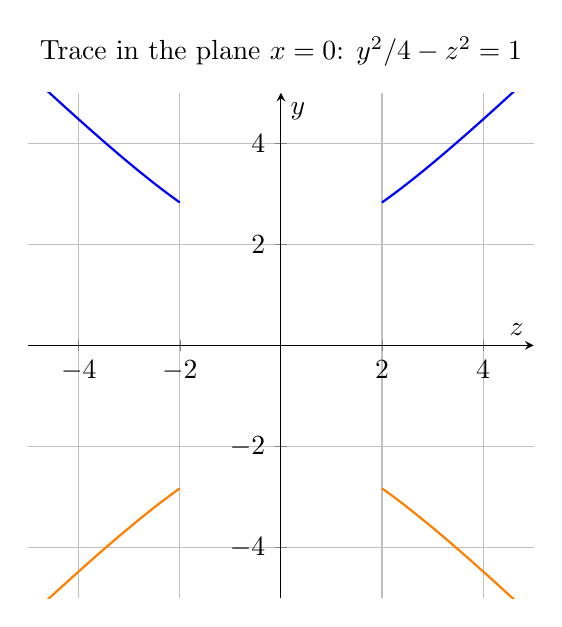
\begin{tikzpicture}
\begin{axis}[
    width=9cm,
    height=8cm,
    xlabel=$z$,
    ylabel=$y$,
    title={Trace in the plane $x=0$: $y^2/4-z^2=1$},
    xmin=-5, xmax=5,
    ymin=-5, ymax=5,
    axis lines=center,
    grid=major,
    axis equal image,
    domain=2:5,
    samples=200
]
\addplot[blue, thick] ({x}, {2*sqrt(1+x^2/4)});
\addplot[blue, thick] ({-x}, {2*sqrt(1+x^2/4)});
\addplot[orange, thick] ({x}, {-2*sqrt(1+x^2/4)});
\addplot[orange, thick] ({-x}, {-2*sqrt(1+x^2/4)});
\end{axis}
\end{tikzpicture}
\end{document}